% This must be in the first 5 lines to tell arXiv to use pdfLaTeX, which is strongly recommended.
\pdfoutput=1
% In particular, the hyperref package requires pdfLaTeX in order to break URLs across lines.

\documentclass[11pt]{article}

% Remove the "review" option to generate the final version.
\usepackage[]{latex/acl}

% Standard package includes
\usepackage{times}
\usepackage{latexsym}
\usepackage{graphicx}

% For proper rendering and hyphenation of words containing Latin characters (including in bib files)
\usepackage[T1]{fontenc}
% For Vietnamese characters
% \usepackage[T5]{fontenc}
% See https://www.latex-project.org/help/documentation/encguide.pdf for other character sets

% This assumes your files are encoded as UTF8
\usepackage[utf8]{inputenc}

% This is not strictly necessary, and may be commented out,
% but it will improve the layout of the manuscript,
% and will typically save some space.
\usepackage{microtype}

% This is also not strictly necessary, and may be commented out.
% However, it will improve the aesthetics of text in
% the typewriter font.
\usepackage{inconsolata}
\usepackage{stfloats}

% If the title and author information does not fit in the area allocated, uncomment the following
%
%\setlength\titlebox{<dim>}
%
% and set <dim> to something 5cm or larger.

\title{Avoiding Perjury of Large Language Models using Retrieval Augmentation?}

% Author information can be set in various styles:
% For several authors from the same institution:
% \author{Author 1 \and ... \and Author n \\
%         Address line \\ ... \\ Address line}
% if the names do not fit well on one line use
%         Author 1 \\ {\bf Author 2} \\ ... \\ {\bf Author n} \\
% For authors from different institutions:
% \author{Author 1 \\ Address line \\  ... \\ Address line
%         \And  ... \And
%         Author n \\ Address line \\ ... \\ Address line}
% To start a separate ``row'' of authors use \AND, as in
% \author{Author 1 \\ Address line \\  ... \\ Address line
%         \AND
%         Author 2 \\ Address line \\ ... \\ Address line \And
%         Author 3 \\ Address line \\ ... \\ Address line}

\author{Tomás Vergara Browne \\
  Pontificia Universidad Católica de Chile \\
  \texttt{tomvergara@uc.cl} \\}

\begin{document}
\maketitle
\begin{abstract}
  Retrieval Augmentation provides the abilities to Large Language Models to access external information for them to generate more factual answers. Although the use of Retrieval Augmentation techniques has been intensely studied in the last year, a particular domain of legal domains has not been significantly studied, in comparison to other domains. In this paper, we explore the use of Retrieval Augmentation for the Mistral 7B model, which has surprised the open source community for its ability to supersede in performance models which are considerably larger. Through the use of the open source tools in LangChain, we are able to add retrieval capabilities to the model. With this model, we are might be able to a strong evaluation benchmark of LexGLUE. We were not able to achieve results as strong as the baselines for LexGLUE. This was mostly due to the lack of several naive choices, which can be easily improved upon. Due to time restrictions on the deadline, we were not able to continue improving upon these results. We make our code publicly available for reproducibility and auditability of the results.\footnote{\href{https://github.com/tvergara/RAG-Lawyer}{https://github.com/tvergara/RAG-Lawyer}}
\end{abstract}

\section{Introduction}
Retrieval Augmented Generation (RAG) is a technique to combine information retrieval, with a text generator. I has been extensively studied over this last year the use of RAG with Large Language Models (LLMs), showing that it can substantially improve a model's performance \cite{ram2023context}. One particular aspect that this technique is allowing to improve is the models factuallity of its answers \cite{lewis2020retrieval}.

Altough there has been some exploration on the use of LLMs in the legal domain \cite{chalkidis2020legal}, there has not been that much focus on the use of RAG techniques to enhance a model's abilities to perform on standarized legal benchmarks, such as LexGLUE \cite{chalkidis-etal-2022-lexglue}. For example, \cite{savelka2023explaining} uses a RAG technique with GPT-4 and empirically shows that it makes the model less prone to hallucinations and provides more factual answers when explaining legal concepts.

Also, the model Mistral 7B \cite{jiang2023mistral} has arised as a potential state of the art in relatively small open source LLMs. It is able to outperform much bigger models in many domains, such as Llama 2 with 30B \cite{touvron2023llama}.

\begin{table*}[t]
\centering
\begin{tabular}{l|c|c|c|c|c|c}
  \textbf{Dataset} & \textbf{ECtHR A} & \textbf{ECtHR B} & \textbf{SCOTUS} \\
\hline
\textbf{Model} & \(\mu\)-F1 / m-F1 & \(\mu\)-F1 / m-F1 & \(\mu\)-F1 / m-F1 \\
\hline
TFIDF+SVM & 62.6 / 48.9 & 73.0 / 63.8 & 74.0 / 64.4 \\
BERT & 71.2 / 63.6 & 79.7 / 73.4 & 68.3 / 58.3 \\
RoBERTa & 69.2 / 59.0 & 77.3 / 68.9 & 71.6 / 62.0 \\
DeBERTa & 70.0 / 60.8 & 78.8 / 71.0 & 71.1 / 62.7 \\
Longformer & 69.9 / 64.7 & 79.4 / 71.7 & 72.9 / 64.0 \\
BigBird & 70.0 / 62.9 & 78.8 / 70.9 & 72.8 / 62.0 \\
Legal-BERT & 70.0 / 64.0 & 80.4 / 74.7 & 76.4 / 66.5 \\
CaseLaw-BERT & 69.8 / 62.9 & 78.8 / 70.3 & 76.6 / 65.9 \\
  \textbf{RAG-Lawyer} & \textbf{45.1 / 38.6} & \textbf{45.5 / 39.1} & \textbf{34.6 / 21.0}\\
\hline
\end{tabular}
\caption{Performance comparison of RAG-Lawyer to baselines.}
\end{table*}
This calls for the natural approach of combining RAG and Mistral 7B, into the LexGLUE benchmark. Considering the advances that this model and RAG can make in performance, it is not unrealistic to aim for a new state of the art in the LexGLUE benchmark.
\section{Related Work}
\subsection{LLMs in the legal domain}
There has been much work into fine tuning models for the legal domain. One particular example is LEGAL-BERT  \cite{chalkidis2020legal}. This model currently holds the state-of-the-art in the LexGLUE benchmark.
\subsection{RAG in the legal domain}
There has been some work into the use of RAG techniques in the legal domain. For example, \cite{savelka2023explaining} uses a RAG technique with GPT-4 and empirically shows the model provides more factual answers when explaining legal concepts.
\section{Methods}
We are using the open source framework of \href{https://github.com/langchain-ai/langchain}{LangChain} to implement RAG techniques into open source models. Specifically, we are using the \href{https://github.com/chroma-core/chroma}{ChromaDB} tools inside of LangChain to implement a knowledge base in a vector database.

We are using an embedding based on the model General Text Embeddings (GTE) \cite{li2023towards}. This is an open source embedding model which is currently state-of-the-art in language embeddings benchmarks.


The information in the knowledge base is extracted from the Basic Laws book 2016 edition (found \href{https://www.archives.gov/files/about/laws/basic-laws-book-2016.pdf}{here}), and the European Convention on Human Rights (found \href{https://www.echr.coe.int/documents/d/echr/convention_ENG}{here}).

Instead of Mistral 7B, we decided to jump straight ahead into a finetuned version of the model, to be able to follow instructions much more consistently. This language model was developed by Intel, using the Orca dataset \cite{mukherjee2023orca}, and using DPO \cite{rafailov2023direct}. This model is called \verb|Neural Chat 7B|.

\section{Datasets}
We evaluated on 3 out of the 7 tasks available on LexGLUE. This decision was not a design choice, but rather a miscalculation on the time it took to evaluate each task. When we realized that evaluating on the datasets actually took more than 4 hours in each run, we decided to remain more conservative on the number of tasks to evaluate, but prioritize an ablation study on the tasks, to understand better the effect of RAG techniques on these datasets.

The datasets used were:
\begin{itemize}
    \item \textbf{SCOTUS:} A dataset based on the US Supreme Court cases. It is a single-label multi-class classification task, where given a court opinion, the task is to predict the relevant issue areas.
    \item \textbf{ECtHR (Task A):} A dataset based on the European Court of Human Rights cases. It is a single-label multi-class classification task, where for each case, the dataset provides a list of factual paragraphs (facts) from the case description. Each case is mapped to articles of the ECHR that were violated (if any).
    \item \textbf{ECtHR (Task B):} An updated version of the ECtHR Task A, but with new cases, and also with annotated rationals between cases' facts.
\end{itemize}


\section{Results}

A detailed description of our results can be found on Table 1.


As we can see, the results are far away from the existing baselines, which is underwhelming. In the case of the SCOTUS dataset, out model does not even reach the 50\% of the accuracy reached by any of the other baselines used in the dataset. In the other datasets, our results are much closer, but still very far away to be considered "good" results.

Although these results are not as good as we initially intended, we are not surprised. There is still a ton of work to be done to improve these results. In the discussion section we will delve deep into the details of how these results could be drastically improved.

\section{Ablation study}
We were interested in understanding the importance of the number of chunks retrieved from the knowledge base, into the performance of the model. We chose to do $n \in \{1, 2, 4\}$ number of chunks. Again, these choices were made mostly because running the inference on the tasks is costly in terms of time, so we could not really afford to extend our study to many more values. We did this evaluation in the tasks of the ECtHR. The figure 1 shows the results we obtained.

\begin{figure}
  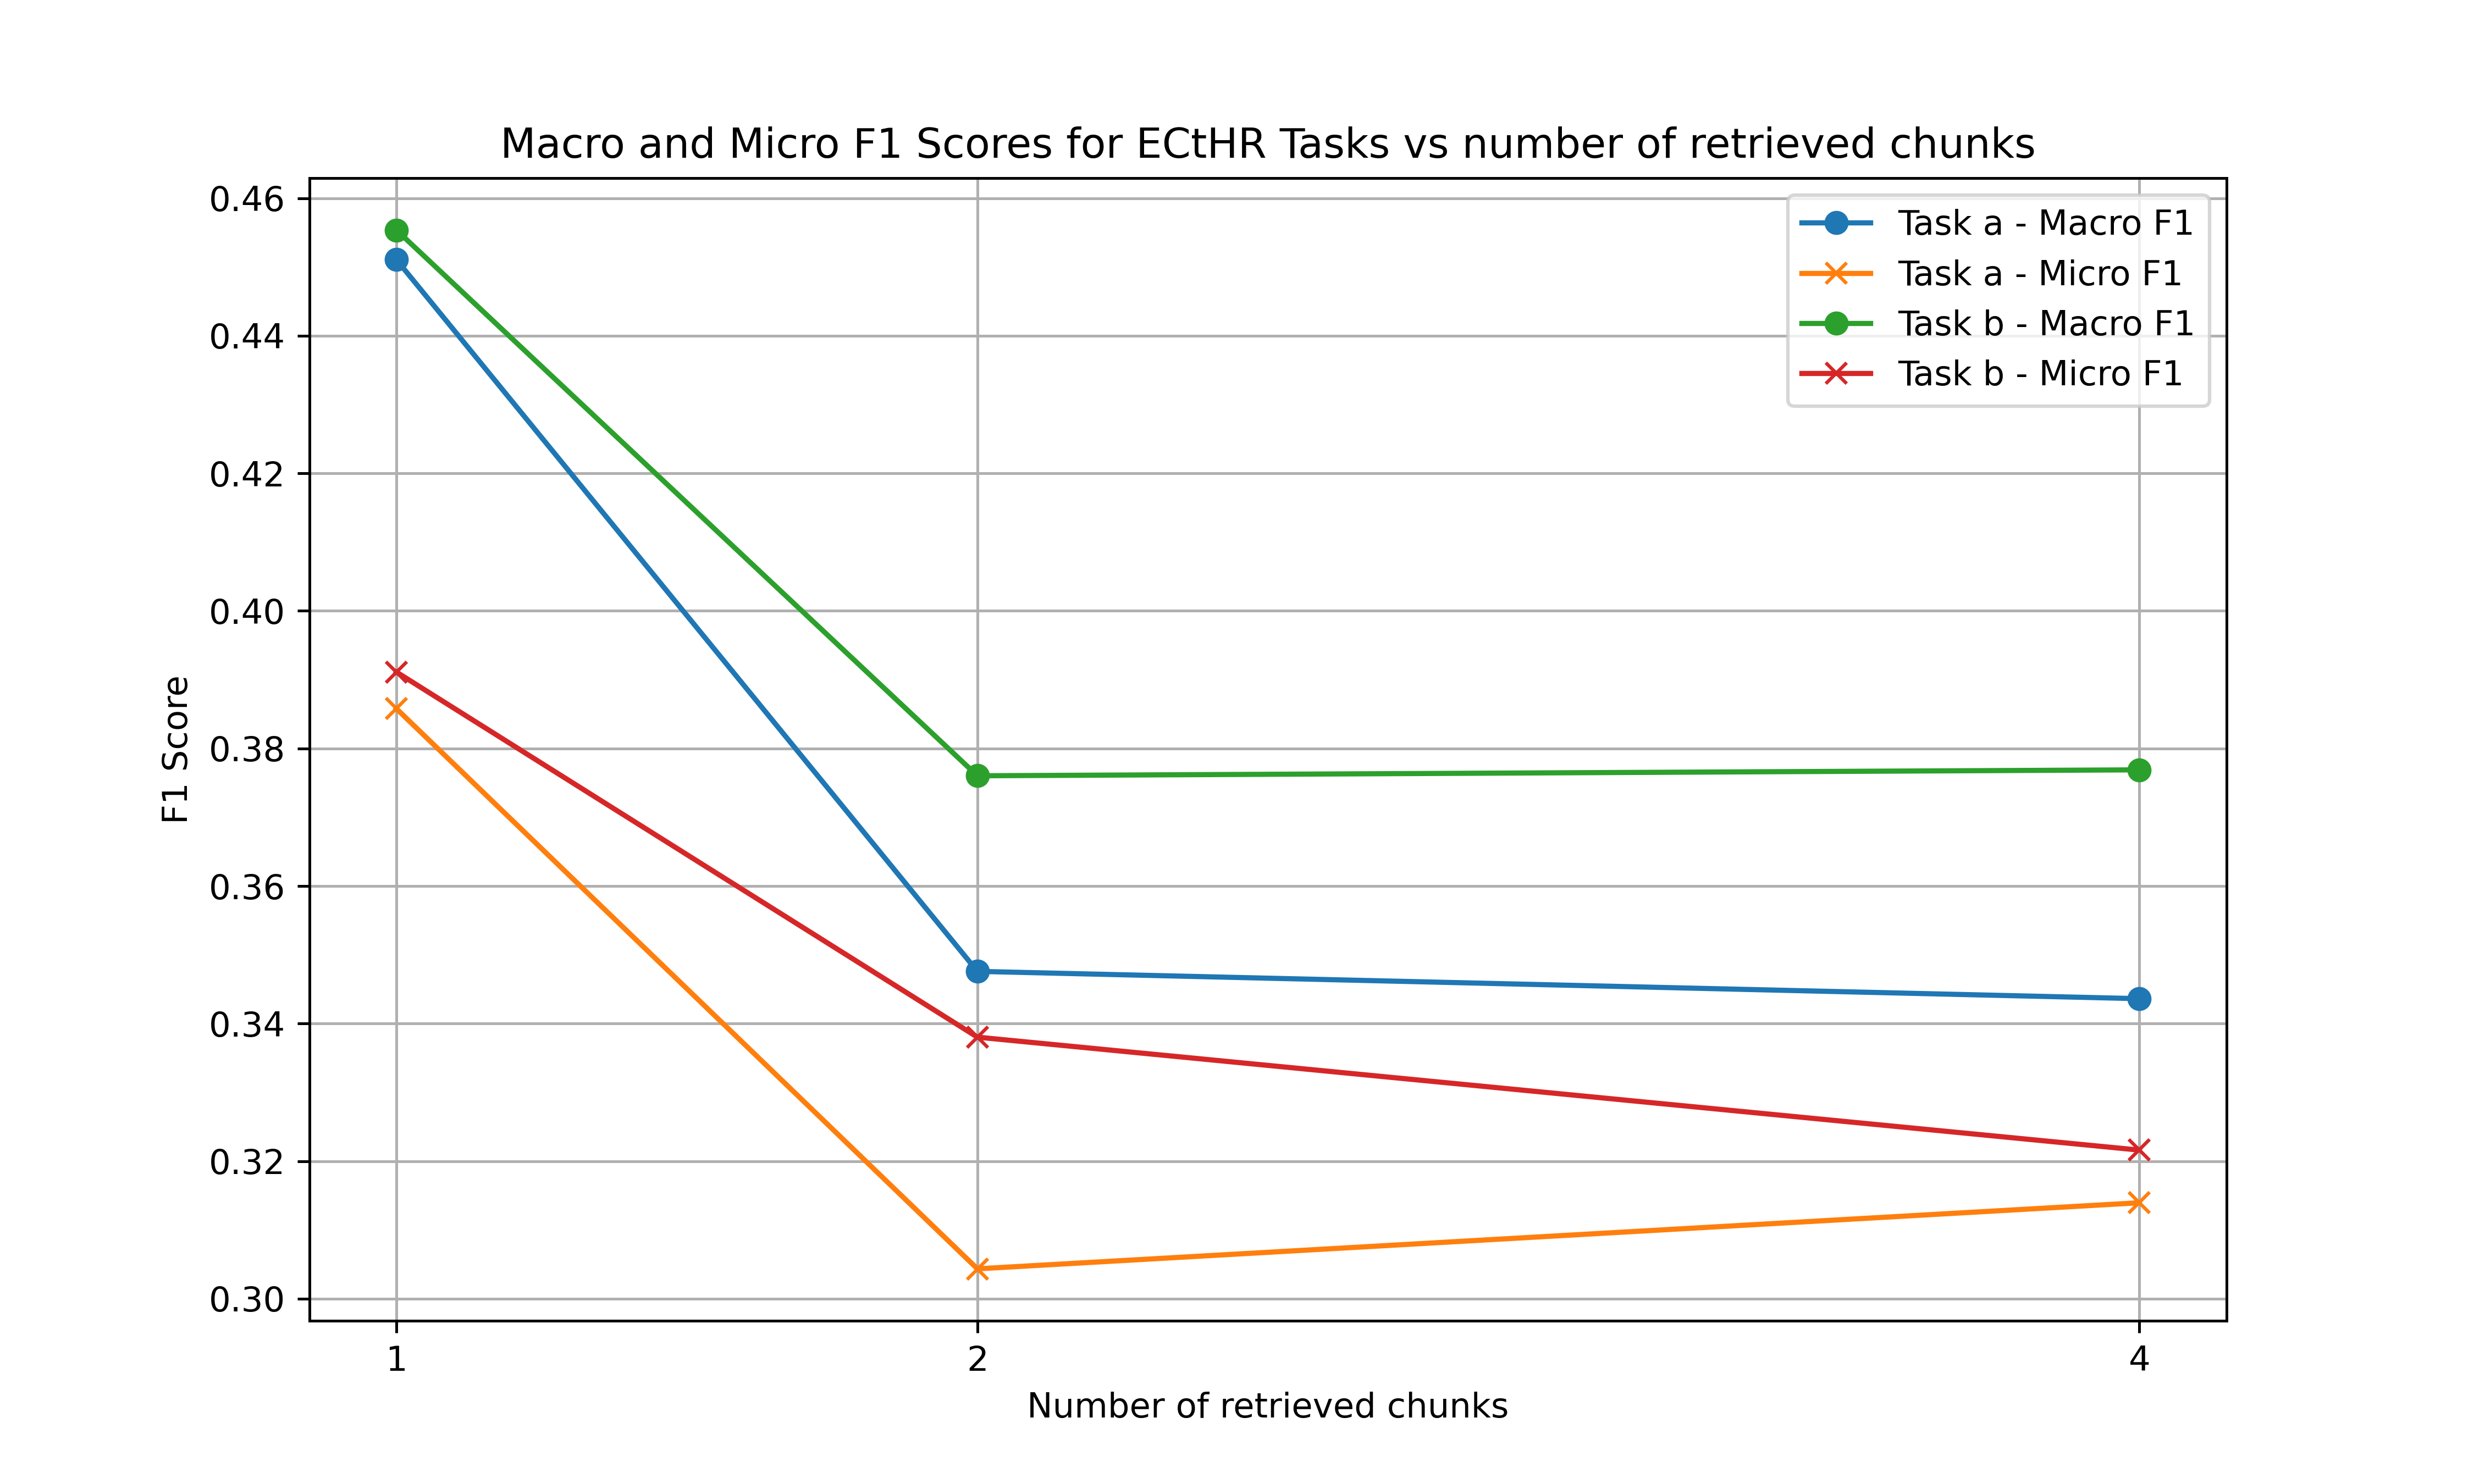
\includegraphics[scale=0.32]{ablation.png}
  \caption{Performance of RAG-Lawyer varying the number of retrieved chunks.}
\end{figure}

One interesting point is that consistently, the most performant number of retrieved chunks is 1. It is entirely possible that the first chunk is the only one particularly relevant for the objective. The ECtHR datasets are prompted to ask if a particular right was effectively violated, so in theory the retrieval process might be just getting the description of that right into memory, and then doing the inference. That way, other context that it is added later is much less necessary in comparison to the first chunk. The extra chunks might end up adding noise to the prompt, making it have a worse prediction.

\section{Discussion}
Although current results are not promising, we made several choices that we believe to be severely limiting the potential of the model using RAG techniques. A non extensive list of \textit{improvable} choices are:
\begin{itemize}
  \item \textbf{Prompts}: The prompts were very naively designed, and not very calibrated at all. Additionally we could try more techniques such as \textit{Chain-of-thought} \cite{wei2022chain} to elicit explicit reasoning.
  \item \textbf{External knowledge}: Again, the external knowledge bases were very naively chosen, and might be further optimized. In particular, the Basic Laws (2016) book has information which is very general in terms of legal reasoning, and is hard to extract chunks of information that may be useful for the tasks.
  \item \textbf{Complete context}: Due to GPU memory constraints in the IALab cluster, actually fitting all the context of the legal cases into a single forward pass of the model was not feasible. We had to truncate the context to 1000 tokens only, which ignores a lot of information which is potentially useful to the tasks.
  \item \textbf{In depth analysis of chunk size}: Naively, the chunk size was by default chosen to be 100 characters, and this was never then tried with another value.
\end{itemize}


Again, these decisions were far from perfect, and were planned for them to be fixed. However, we underestimated the development time that took to be able to run a 7B model in the cluster, without problems of storage or GPU memory. This significantly set back our development much into the final ours of the deadline.

We still expect to be able to reach competent results by using a finetuned version of Mistral 7B, with RAG techniques. However, we did notice a mistake in our initial beliefs. Initially, we thought that legal benchmarks mostly rely on the recall of factual associations regarding different laws around the world. However, what we found is that these datasets tended to evaluate \textit{legal reasoning} much more than \textit{legal recall}. In this sense, RAG techniques do not show as an important of an improvement as we initially expected. Despite that, considering the strength of Mistral 7B, it can probably reach good results in LexGLUE, even without RAG techniques (just with some manual iteration to get a performant prompt).

\section{Conclusion}
In this work, we present the results of evaluating a finetuned version of Mistral 7B (Neural Chat 7B) on 3 out of the 7 tasks of LexGLUE, using RAG techniques. We found that our results are considerably worse than the existing baselines, but we expect this to be mostly due to the lack of optimization in various design choices made (prompts, external knowledge documents, context given, chunk size chosen). We do find an interesting result, in that the optimal number of chunks retrieved from the external knowledge is consistently 1, maybe indicating that additional chunks may be adding more noise than information.


% Entries for the entire Anthology, followed by custom entries
\bibliography{anthology,custom}

\appendix

\section{Appendix}


\begin{table}[h]
\centering
\begin{tabular}{|c|c|c|c|}
\hline
Task & n & Macro-F1 & Micro-F1 \\
\hline
ECtHR-a & 1 & 45.11 & 38.58 \\
ECtHR-a & 2 & 34.76 & 30.43 \\
ECtHR-a & 4 & 34.36 & 31.40 \\
ECtHR-b & 1 & 45.54 & 39.11 \\
ECtHR-b & 2 & 37.60 & 33.80 \\
ECtHR-b & 4 & 37.69 & 32.16 \\
\hline
\end{tabular}
\caption{Macro and Micro F1 scores for RAG-Lawyer with different number of chunks retrieved}
\label{tab:my_label}
\end{table}
\end{document}
